\documentclass[12,french]{report}
\usepackage{geometry}
\geometry{vmargin=3cm, hmargin=3cm}
\usepackage[T1]{fontenc}
\usepackage[utf8]{inputenc}
\usepackage[french]{babel}
\usepackage{graphicx}
\usepackage{amsmath}
\usepackage{amssymb}
\usepackage{sectsty}
\usepackage{authblk}
\usepackage{algpseudocode}
\usepackage{algorithm}
\usepackage{xspace}
\usepackage{mathtools}
\usepackage{mathrsfs}
\usepackage{enumitem}
\usepackage{titlesec}
\usepackage{hyperref}
\usepackage{xcolor}
\usepackage[justification=centering]{caption}
\usepackage{float}
\usepackage{tabto}

\usepackage{listings}
\usepackage{cleveref}

\renewcommand{\lstlistingname}{Code}
%\renewcommand{\figurename}{Fig.}

\lstdefinestyle{chstyle}{%
backgroundcolor=\color{gray!12},
basicstyle=\ttfamily\small,
showstringspaces=false,
numbers=left}

%\AddThinSpaceBeforeFootnotes
%\FrenchFootnotes

\titleformat{\chapter}[hang]{\bf\Huge}{\thechapter.}{2pc}{}
\titlespacing*{\chapter}{10pt}{0pt}{40pt}[0pt]
\newcommand{\HRule}{\rule{\linewidth}{0.5mm}}

\providecommand{\keywords}[1]{\textbf{\textit{Keywords:}} #1}
\bibliographystyle{apalike}

\usepackage{hyperref}

\begin{document}
\hypersetup{pdfborder=0 0 0}

\begin{titlepage}

\begin{center}
	\vspace*{\stretch{1}}
	\textsc{{\LARGE Institut national des sciences appliquées de Rouen} \\ 			\vspace{6mm} {\Large INSA de Rouen}} \\
	\vspace{5mm}
	
\includegraphics[width=0.4\textwidth]{./Images/insa}\\[1.0 cm]

	\textsc{\Large Projet MSRO GM3 - Vague 2 - Sujet 3}\\[0.6cm]

	% Title
	\HRule \\[0.1cm]
	{ \Huge \bfseries Traitement du signal \\ Etude de deux filtres linéaires}\\[0.2cm]
	\HRule \\[0.95cm]

	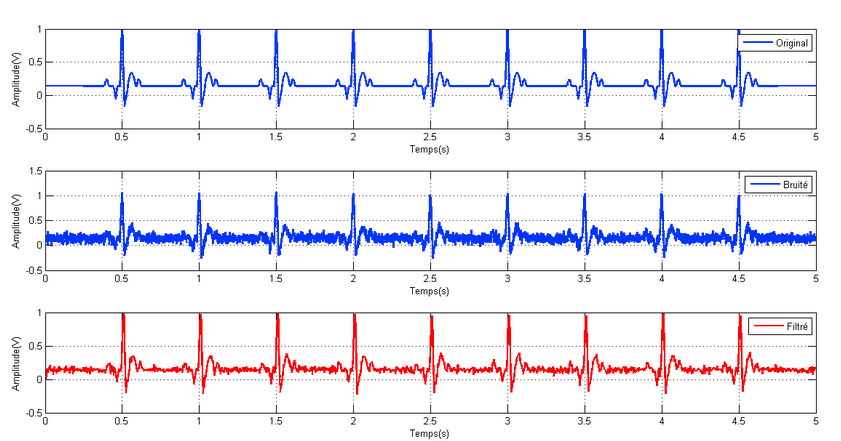
\includegraphics[width=0.8\textwidth]{./Images/Page_de_garde}\\[0.9 cm]

	% Author and supervisor
	\begin{minipage}{0.4\textwidth}
		\begin{flushleft} \large
			\emph{Auteurs:}\\
			Thibaut \textsc{André-Gallis} \\
			{\small\href{mailto:thibaut.andregallis@insa-rouen.fr}{thibaut.andregallis@insa-rouen.fr}} \\
			Kévin \textsc{Gatel} \\
			{\small\href{mailto:kevin.gatel@insa-rouen.fr}{kevin.gatel@insa-				rouen.fr}}
		\end{flushleft}
	\end{minipage}
	\begin{minipage}{0.4\textwidth}
		\begin{flushright} \large
			\emph{Enseignant:} \\
			Natalie \textsc{Fortier} \\
			{\small\href{mailto:natalie.fortier@insa-rouen.fr}								{natalie.fortier@insa-rouen.fr}}
		\end{flushright}
	\end{minipage}
	\vspace*{\stretch{1}}

	\vfill
	{\large 11 Avril 2021}
\end{center}
\end{titlepage}

\tableofcontents

%\listoffigures

\renewcommand{\chaptername}{}
\chapter*{Introduction du problème}

Soit deux filtres $h_k$ et $g_k$ tels que :\\

$$ H(z) = \frac{0.3-0.2z^{-1}+0.4z^{-2}}{1+0.9z^{-1}+0.8z^{-2}} $$
$$ G(z) = \frac{0.2-0.5z^{-1}+0.3z^{-2}}{1+0.7z^{-1}+0.85z^{-2}} $$ \\

Dans un premier temps, on cherche à savoir si ces deux filtres sont réalisables physiquement.\\

On s’intéressera ensuite à la mise en cascade de ces deux filtres pour déterminer s'il agit par équivalence d'un unique filtre.\\

Enfin nous étudierons leur mise en parallèle avec les mêmes objectifs que pour la mise en cascade.


\chapter{Filtres réalisables ?}

\section{Pôles}

\subsection{$H(z)$}

\vspace{0.25cm}

On a $$ H(z) = \frac{0.3-0.2z^{-1}+0.4z^{-2}}{1+0.9z^{-1}+0.8z^{-2}} = \frac{0.3z^2-0.2z+0.4}{z^2+0.9z+0.8} $$

Dénominateur : $$ D_h= z^2+0.9z+0.8 $$

D'où : $$ \begin{array}{ccl}
\Delta & = & 0.9^2-4*1*0.8 \\
	   & = & -2.39 \\
\end{array} $$

On obtient :
$$\left.\begin{aligned}
	&z_{1Dh} = \frac{-0.9+i\sqrt{2,39}}{2} \\
	&\quad\quad = -0.45 + i\frac{\sqrt{2,39}}{2} \\
\end{aligned}\quad\right|
\quad\left.\begin{aligned}
	&z_{2Dh} = \frac{-0.9-i\sqrt{2,39}}{2}\\
	&\quad\quad = -0.45 - i\frac{\sqrt{2,39}}{2} \\
\end{aligned}\right.$$

Ainsi :
$$ |z_{1Dh}|=|z_{2Dh}|=\sqrt{(-0.45)^2+\left(\frac{\sqrt{2,39}}{2}\right)^2} \simeq 0.89 < 1 $$


$H(z)$ a tous ses pôles à l'intérieur du cercle unité \textbf{donc le filtre est réalisable physiquement}.\\

\subsection{$G(z)$}

\vspace{0.25cm}

On a $$ G(z) = \frac{0.2-0.5z^{-1}+0.3z^{-2}}{1+0.7z^{-1}+0.85z^{-2}} = \frac{0.2z^2-0.5z+0.3}{z^2+0.7z+0.85} $$

Dénominateur : $$ D_g= z^2+0.7z+0.85 $$

D'où : $$ \begin{array}{ccl}
\Delta & = & 0.7^2-4*1*0.85 \\
	   & = & -2.91 \\
\end{array} $$

On obtient :
$$\left.\begin{aligned}
	&z_{1Dg} = \frac{-0.7+i\sqrt{2,91}}{2} \\
	&\quad\quad = -0.35 + i\frac{\sqrt{2,91}}{2} \\
\end{aligned}\quad\right|
\quad\left.\begin{aligned}
	&z_{2Dg} = \frac{-0.7-i\sqrt{2,91}}{2}\\
	&\quad\quad =-0.35 - i\frac{\sqrt{2,91}}{2} \\
\end{aligned}\right.$$

Ainsi :
$$ |z_{1Dg}|=|z_{2Dg}|=\sqrt{(-0.35)^2+\left(\frac{\sqrt{2,91}}{2}\right)^2} \simeq 0.92 < 1 $$


$G(z)$ a tous ses pôles à l'intérieur du cercle unité \textbf{donc le filtre est réalisable physiquement}.

\section{Zéros}

\subsection{$H(z)$}

\vspace{0.25cm}

On a $$ H(z) = \frac{0.3z^2-0.2z+0.4}{(z-z_{1Dh})(z-z_{2Dh})} $$

Numérateur : $$ N_h= 0.3z^2-0.2z+0.4 $$

D'où : $$ \begin{array}{ccl}
\Delta & = & (-0.2)^2-4*0.3*0.4 \\
	   & = & -0,44 \\
\end{array} $$

On obtient :
$$\left.\begin{aligned}
	&z_{1Nh} = \frac{0.2+i\sqrt{0.44}}{2*0.3} \\
	&\quad\quad = \frac{1}{3} + \frac{5}{3}i\sqrt{0.44} \\
\end{aligned}\quad\right|
\quad\left.\begin{aligned}
	&z_{2Nh} = \frac{0.2-i\sqrt{0.44}}{2*0.3}\\
	&\quad\quad = \frac{1}{3} - \frac{5}{3}i\sqrt{0.44} \\
\end{aligned}\right.$$

\subsection{$G(z)$}

\vspace{0.25cm}

On a $$ G(z) = \frac{0.2z^2-0.5z+0.3}{(z-z_{1Dg})(z-z_{2Dg})} $$

Numérateur : $$ N_g= 0.2z^2-0.5z+0.3 $$

D'où : $$ \begin{array}{ccl}
\Delta & = & (-0.5)^2-4*0.2*0.3 \\
	   & = & 0.01 \\
\end{array} $$

On obtient :
$$\left.\begin{aligned}
	&z_{1Ng} = \frac{0.5+\sqrt{0.01}}{2*0.2} \\
	&\quad\quad = \frac{3}{2} \\
\end{aligned}\quad\right|
\quad\left.\begin{aligned}
	&z_{2Ng} = \frac{0.5-\sqrt{0.01}}{2*0.2}\\
	&\quad\quad = 1 \\
\end{aligned}\right.$$\\

\section{Représentation dans le plan complexe (zplane)}

\vspace{0.25cm}
On a :
$$ H(z) = \frac{(z-z_{1Nh})(z-z_{2Nh})}{(z-z_{1Dh})(z-z_{2Dh})} $$

et
$$ G(z) = \frac{(z-z_{1Ng})(z-z_{2Ng})}{(z-z_{1Dg})(z-z_{2Dg})} $$

\begin{figure}[H]
    \begin{minipage}[c]{.50\linewidth}
        \centering
        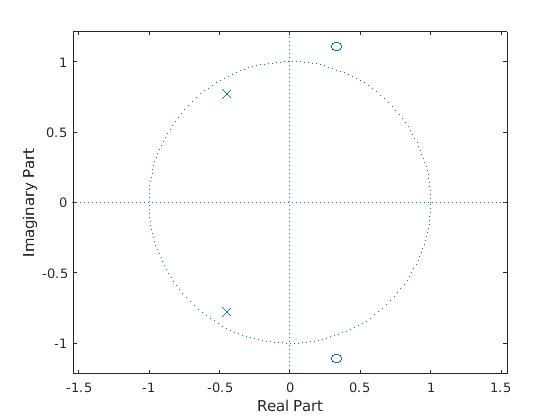
\includegraphics[width=1\textwidth]{./Images/zplane_H}\\
        \caption{Visualisation des pôles et des zéros du filtre $H$}
    \end{minipage}
    \hfill%
    \begin{minipage}[c]{.50\linewidth}
        \centering
        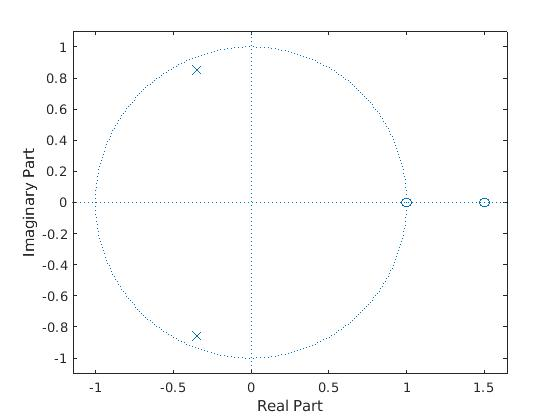
\includegraphics[width=1\textwidth]{./Images/zplane_G}\\
        \caption{Visualisation des pôles et des zéros du filtre $G$}
    \end{minipage}
\end{figure}\vspace{0.3cm}

\section{Réponse en fréquence}

\begin{figure}[H]
    \begin{minipage}[c]{.50\linewidth}
        \centering
        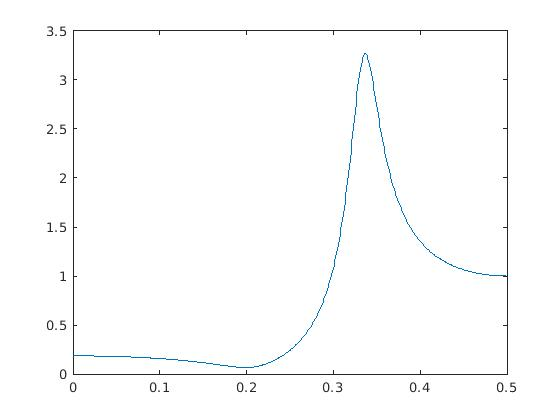
\includegraphics[width=1\textwidth]{./Images/freqz_H}\\
        \caption{Visualisation de $|H(f)|$ sur [0,0.5]}
    \end{minipage}
    \hfill%
    \begin{minipage}[c]{.50\linewidth}
        \centering
        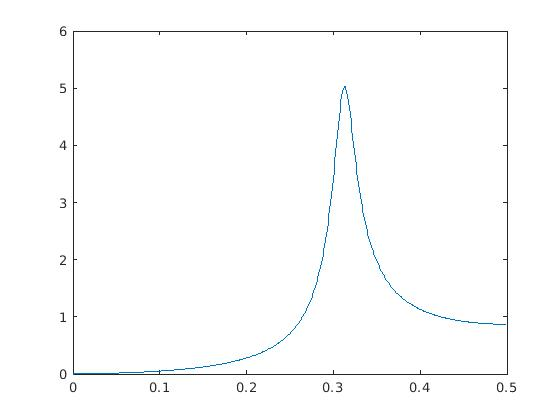
\includegraphics[width=1\textwidth]{./Images/freqz_G}\\
        \caption{Visualisation de $|G(f)|$ sur [0,0.5]}
    \end{minipage}
\end{figure}\vspace{0.3cm}


\chapter{Mise en cascade}

On met en cascade les filtres $H(z)$ et $G(z)$. Posons $y_k$ le filtre équivalent à la convolutée tel que : 
$$y_k=h_k*g_k$$

On a :
$$ Y(z)=\sum_{k=-\infty}^{\infty}y_kz^{-k}=\sum_{k=-\infty}^{\infty}\left(\sum_{m=-\infty}^{\infty}h_mg_{k-m}\right)z^{-k} $$

On pose $n=k-m$

$$ Y(z)=\sum_{n=-\infty}^{\infty}\left(\sum_{m=-\infty}^{\infty}h_mg_n\right)z^{-(n+m)} $$
$$ Y(z)=\sum_{n=-\infty}^{\infty}\left(\sum_{m=-\infty}^{\infty}h_mz^{-m}\right)g_nz^{-n} $$

On retrouve
$$ Y(z)=H(z)G(z) $$

Le filtre équivalent à la mise en cascade des deux filtres est le produit des deux filtres.\\

On a donc \\
$$ Y(z)= \frac{(z-z_{1Nh})(z-z_{2Nh})}{(z-z_{1Dh})(z-z_{2Dh})}*\frac{(z-z_{1Ng})(z-z_{2Ng})}{(z-z_{1Dg})(z-z_{2Dg})} $$\\
$$Y(z)= \frac{0.3-0.2z^{-1}+0.4z^{-2}}{1+0.9z^{-1}+0.8z^{-2}}*\frac{0.2-0.5z^{-1}+0.3z^{-2}}{1+0.7z^{-1}+0.85z^{-2}} $$\\

En développant on trouve :
$$Y(z)=\frac{0.06-0.19z^{-1}+0.27z^{-2}-0.26z^{-3}+0.12z^{-4}}{1+1.6z^{-1}+2.28z^{-2}+1.325z^{-3}+0.68z^{-4}} $$\\

On peut ainsi représenter les pôles et les zéros de ce filtre sur le plan complexe comme ci-dessous :

\begin{figure}[H]
	\center
	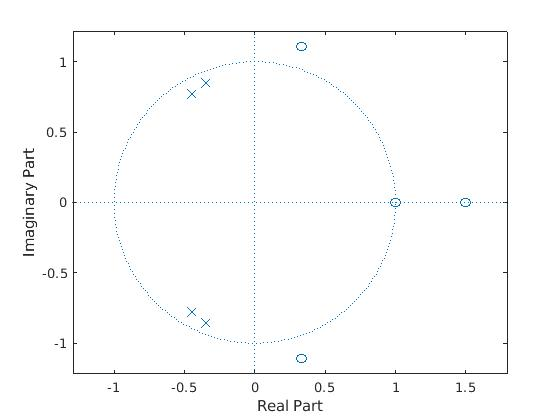
\includegraphics[width=0.6\textwidth]{./Images/zplane_HG}
	\caption{Visualisation des pôles et des zéros du filtre $Y$}
\end{figure}\vspace{0.2cm}

On retrouve bien les deux pôles et les deux zéros des filtres respectifs $H$ et $G$.\\

On peut également visualiser sa réponse en fréquence ci-dessous :

\begin{figure}[H]
	\center
	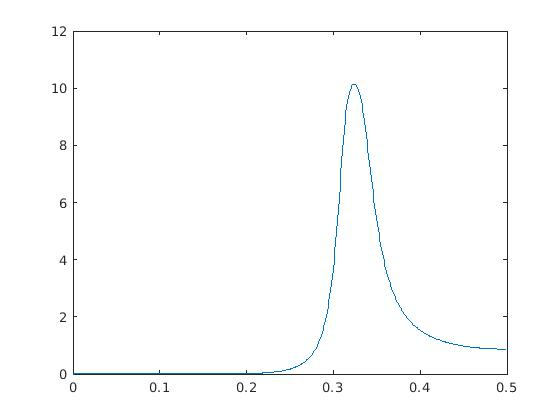
\includegraphics[width=0.6\textwidth]{./Images/freqz_HG}
	\caption{Visualisation de $|Y(f)|$ sur [0,0.5]}
\end{figure}\vspace{0.2cm}

\chapter{Mise en parallèle}


\chapter*{Conclusion}
\addcontentsline{toc}{chapter}{Conclusion}



\chapter*{Annexe}
\addcontentsline{toc}{chapter}{Annexe}



\end{document}
